% Texfile pre projekt 3 z Typografie a publikovani
% Autor: Marek Marusic
% Email: xmarus05@stud.fit.vutbr.cz
\documentclass[11pt,a4paper,titlepage]{article}

\usepackage{times}
\usepackage[left=2cm,text={17cm,24cm},top=3cm]{geometry}
\usepackage[czech]{babel}
\usepackage[utf8]{inputenc}
\usepackage[IL2]{fontenc}
\usepackage{multirow}
\usepackage[ruled,czech,linesnumbered,longend,noline]{algorithm2e}
\usepackage{graphics}
\usepackage{picture}
\usepackage{algorithmic}

\begin{document}
\begin{titlepage}

\begin{center}
\Huge\textsc{Vysoké učení technické v~Brně \\
\huge Fakulta informačních technologií\\}

\vspace{\stretch{0.382}}
\LARGE Typografie a~publikování \,--\,3.\,projekt \\
\Huge{Tabulky a~obrázky} \\
\vspace{\stretch{0.618}}
\end{center}
{\Large \today \hfill
Marek Marušic}
\end{titlepage}

\section{Úvodní strana}
Název práce umístěte do zlatého řezu a~nezapomeňte uvést dnešní datum a~vaše jméno a~příjmení.

\section{Tabulky}
Pro sázení tabulek můžeme použít buď prostředí \texttt{ tabbing } nebo prostředí \texttt{ tabular.}

\subsection{Prostředí \texttt{ tabbing }}
Při použití \texttt{ tabbing } vzpadá tabulka následovne:
\begin{tabbing}
Ovoce \qquad\qquad\= cena \qquad
\= monžství \kill
\bfseries Ovoce \>
\bfseries Cena \>
\bfseries Množství \\
Jablka \> 25,90 \> 3\,kg\\
Hrušky \> 27,40 \> 2,5\,kg\\
Vodní melouny \> 35,-- \> 1\,ks\\\\
\end{tabbing}
Toto prostředí se dá také pužít pro sázení \texttt{ algoritmů }, ovšem vhodnější je použít prostředí algorithm nebo 
\texttt{ algorthme2e } (viz sekce \ref{sec:Algoritmy}).

\subsection{Prostředí \texttt{tabular}}
Další možností, jak vytvořit tabulku, je použít prostředí \texttt{tabular}. Tabulky pak budou vypadat takto\footnote{Kdyby byl problem s~\texttt{cline,} zkuste se podívat třeba sem: http://www.abclinuxu.cz/tex/poradna/show/325037}:

\begin{table}[ht]
\catcode`\-=12
\begin{center}
\begin{tabular}{|c|c|c|}
\hline
 & \multicolumn{2}{|c|}{\bfseries Cena}\\ \cline{2-3}
\bfseries Měna & \bfseries nákup & \bfseries prodej\\ \hline
EUR & 27,34 & 27,42\\
GBP & 33,09 & 33,21\\
USD & 19,87 & 19,95\\ \hline
\end{tabular}

\caption{Tabulka kurzů k~dnešnímu dni}
\label{tab:kurz}
\end{center}
\end{table}


\begin{table}[ht]
\catcode`\-=12
\begin{center}
\begin{tabular}{|c|c|}
\hline
A & $\lnot A$ \\ \hline
\bfseries P & N \\ \hline
\bfseries O & O\\ \hline
\bfseries X & X \\ \hline 
\bfseries N & P \\ \hline
\end{tabular}
\begin{tabular}{|c|c|c|c|c|c|}
\hline
\multicolumn{2}{|c}{\multirow{2}{*}{A $\wedge$ B}}  & \multicolumn{4}{|c|}{ B}\\ \cline{3-6}
\multicolumn{2}{|c|}{} & \textbf P & \textbf O & \textbf X & \textbf N \\ \hline
\multirow{4}{*}{A} & \textbf P & P & O & X & N\\ \cline{2-6}
 & \textbf O & O & O & N & N \\ \cline{2-6}
 & \textbf X & X & N & X & N \\ \cline{2-6}
 & \textbf N & N & N & N & N \\ \hline
\end{tabular}
\begin{tabular}{|c|c|c|c|c|c|}
\hline
\multicolumn{2}{|c}{\multirow{2}{*}{A $\vee$ B}}  & \multicolumn{4}{|c|}{ B}\\ \cline{3-6}
\multicolumn{2}{|c|}{} & \textbf P & \textbf O & \textbf X & \textbf N \\ \hline
\multirow{4}{*}{A} & \textbf P & P & P & P & P\\ \cline{2-6}
 & \textbf O & P & O & P & O \\ \cline{2-6}
 & \textbf X & P & P & X & X \\ \cline{2-6}
 & \textbf N & P & O & X & N \\ \hline
\end{tabular}
\begin{tabular}{|c|c|c|c|c|c|}
\hline
\multicolumn{2}{|c}{\multirow{2}{*}{A $\rightarrow$ B}}  & \multicolumn{4}{|c|}{ B}\\ \cline{3-6}
\multicolumn{2}{|c|}{} & \textbf P & \textbf O & \textbf X & \textbf N \\ \hline
\multirow{4}{*}{A} & \textbf P & P & O & X & N\\ \cline{2-6}
 & \textbf O & P & O & P & O \\ \cline{2-6}
 & \textbf X & P & P & X & X \\ \cline{2-6}
 & \textbf N & P & P & P & P \\ \hline
\end{tabular}
\caption{Protože Kleeneho trojhodnotová logika už je "zastaralá", uvádíme si zde příklad čtyřhodnotové logiky}
\label{tab:tab2}
\end{center}
\end{table}

\section{Algoritmy \label{sec:Algoritmy}}
Pokud budeme chtít vysázet alrgoritmus, můžeme použít prostředí \texttt{algorithm}\footnote{Pro nápovědu, jak zacházet s~prostředím \texttt{algorithm,}můžeme zkusit tuhle stránku:\\
http://ftp.cstug.cz/pub/tex/CTAN/macros/latex/contrib/algorithms/algorithms.pdf.} nebo \texttt{algorithm2e}\footnote{Pro \texttt{algorithm2e} zase tuhle: http://ftp.cstug.cz/pub/tex/CTAN/macros/latex/contrib/algorithm2e/algorithm2e.pdf.}. Příklad použití prostředí \texttt{algorithm2e} viz Algoritmus \ref{alg:1}.
\bigskip

\begin{algorithm}[ht]
\SetKwInput{Input}{Input}
\SetKwInOut{Output}{Output}
\caption{F\small AST\normalsize SLAM}
\label{alg:1}
\SetNlSty{}{}{:  }
\SetInd{1em}{1em}
\SetNlSkip{-1.33em}

\Input{$(X_{t-1},u_t,z_t)$}
\Output{$X_t$}
\BlankLine
\Indp\Indp

$\overline{X_t} = X_t = 0$\\
\For{$k=1 \textnormal{ to } M$}
{
	$x_t^{[k]} = sample\_motion\_model(u_t,x_{t-1}^{[k]})$\\
    $w_t^{[k]} = measurement\_model(z_t,x_t^{[k]},m_{t-1})$\\
    $m_t^{[k]} = updated\_occupancy\_grid(z_t,x_t^{[k]},m_{t-1}^{[k]})$\\
    $\overline{X_t} = \overline{X_t} +\langle x_x^{[k]},w_t^{[m]}\rangle$\\
}
\For{$k=1 \textnormal{ to } M$}
{
	draw $i$ with probability $\approx w_t^{[i]}$ \\
    add $\langle x_x^{[k]},m_t^{[k]} \rangle \textnormal{ to } X_t$\\
}
\Return{$X_t$}
\end{algorithm}

\section{Obrázky}
Do našich článků můžeme samozřejmě vkládat obrázky. Pkoud je obrázkem fotografie, můžeme klidně použít bitmapový soubor. Pokud by to ale mělo být nějaké schéma nebo něco podobného, je dobrým zvykem takovýto brázek vytvořit vektorově.
\begin{figure}[ht]
\center{
\scalebox{0.4}
{   
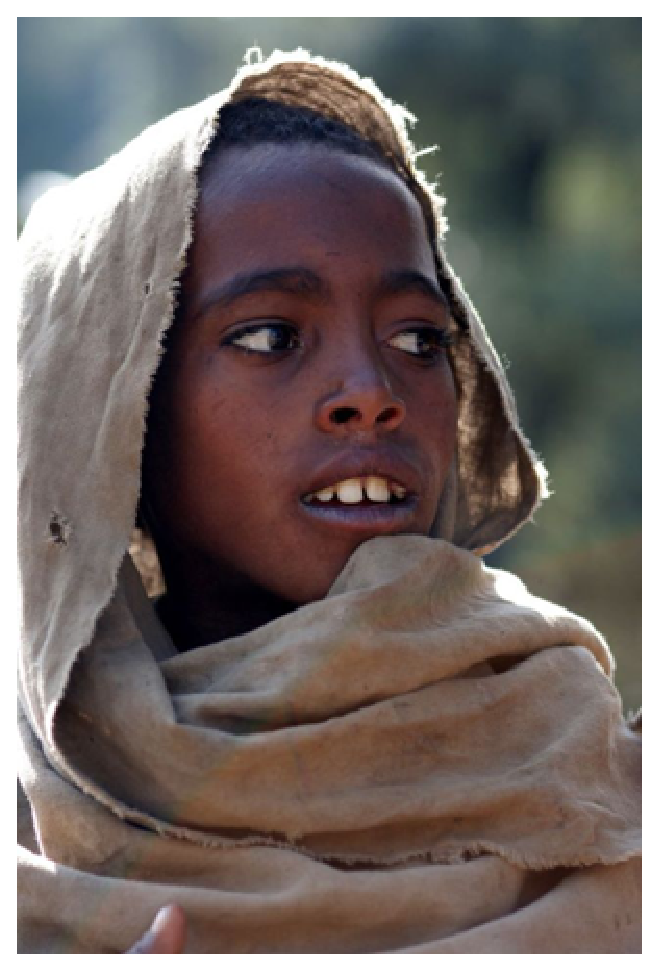
\includegraphics{etiopan.eps}
\reflectbox{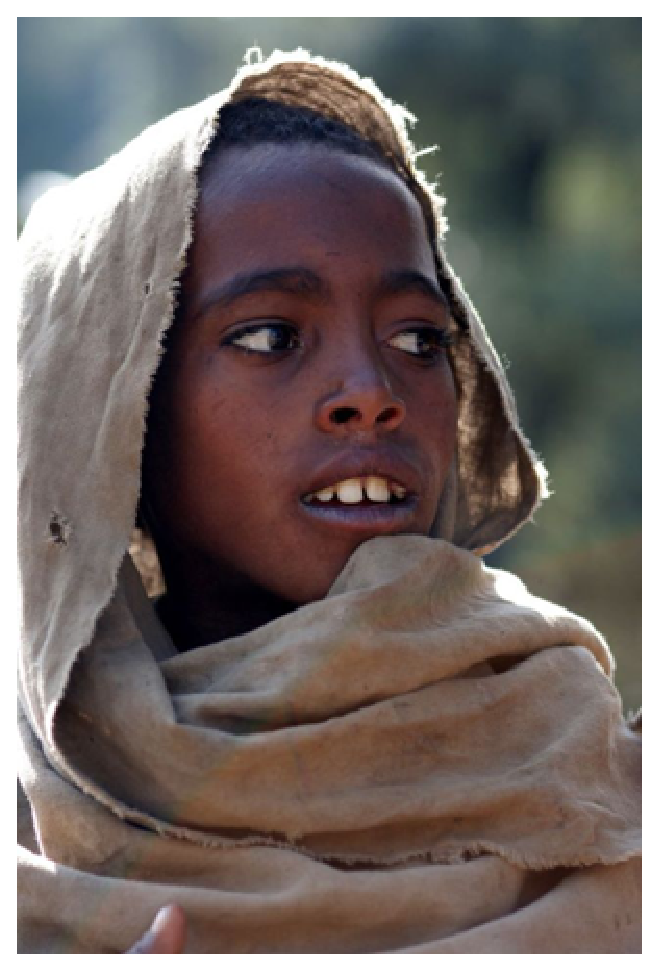
\includegraphics{etiopan.eps}}
}
\caption{Malý etiopánek a~jeho bratříček}
\label{fig:etiopan}}
\end{figure}

\newpage

Rozdíl mezi vektorovým\,\ldots
\begin{figure}[ht]
\begin{center}
\scalebox{0.4}
{
\includegraphics{oniisan.eps}}
\caption{Vektorový obrázek}
\label{fig:Vect}
\end{center}
\end{figure}

\ldots\, a~bitmapovým obrázkem \begin{figure}[ht]
\begin{center}
\scalebox{0.6}
{
\includegraphics{oniisan2.eps}}
\caption{Bitmapový obrázek}
\label{fig:bitmap}
\end{center}
\end{figure}

\noindent se projeví například při zvětšení.

Odkazy (nejen ty) na obrázky \ref{fig:etiopan}, \ref{fig:Vect} a~\ref{fig:bitmap}, na tabulky \ref{tab:kurz} a~\ref{tab:tab2} a~také na algoritmus \ref{alg:1} jsou udělány pomocí křížových odkazů. Pak je ovšem potřeba zdrojový soubor přeložit dvakrát.

Vektorové borázky lze vytvořit přímo v~\LaTeX u, například pomocí prostředí \texttt{picture.} Všechny rozměry jsou uváděny v~mm.

\newpage
\begin{figure}[ht]
\setlength{\unitlength}{4pt}
\begin{picture}(115,158.5)(0,0)
\linethickness{1pt}
\put(0,0){\framebox(115,158.5)}
\put(30,124){\framebox(55,10)}
\put(52,128){\textbf{Hlavička}}
\put(30,35){\framebox(55,75)}
\put(50,72){\textbf{Textové tělo}}
\put(30,10){\framebox(55,10)}
\put(54,14){\textbf{Pata}}
\put(94,80){\framebox(15,10)}
\put(96,86){\textbf{Okrajová}}
\put(95.5,82.5){\textbf{poznámka}}
\linethickness{0.3pt}
\put(112,0){\vector(0,1){158.5}}
\put(112,158.5){\vector(0,-1){158.5}}
\put(0,93){\vector(1,0){15}} 
\put(15,93){\vector(-1,0){15}}
\put(85,93){\vector(1,0){9}}
\put(94,93){\vector(-1,0){9}}
\put(94,93){\vector(1,0){15}}
\put(109,93){\vector(-1,0){15}}
\put(30,137){\vector(1,0){55}}
\put(85,137){\vector(-1,0){55}}
\put(0,3){\vector(1,0){115}}
\put(115,3){\vector(-1,0){115}}
\put(88,144){\vector(0,1){14.5}}
\put(88,158.5){\vector(0,-1){14.5}}
\put(88,134){\vector(0,1){10}}
\put(88,144){\vector(0,-1){10}}
\put(88,124){\vector(0,1){10}}
\put(88,134){\vector(0,-1){10}}
\put(88,110){\vector(0,1){14}}
\put(88,124){\vector(0,-1){14}}
\put(88,35){\vector(0,1){75}}
\put(88,110){\vector(0,-1){75}}
\put(88,20){\vector(0,1){15}}
\put(88,35){\vector(0,-1){15}}
\put(88,10){\vector(0,1){10}}
\put(88,20){\vector(0,-1){10}}
%%%%%
\linethickness{0.2pt}
\put(93,105){\vector(-1,-4){3}}
\put(100,50){\vector(3,2){12}}
\linethickness{0.4pt}
\multiput(15,158.5)(0,-10){16}{\line(0,-1){7}}
\multiput(0,144)(10,0){11}{\line(1,0){7}}
\put(0.5,94.5){Mezera = 15}
\put(97.5,97){Šířka}
\put(95.5,94.5){boxu = 15}
\put(48,138.5){Šířka boxu = 55}
\put(48,4.5){Šířka stránky = 155}
\put(93,153){Výška}
\put(90,150){mezery = 14,5}
\put(93,140){Výška}
\put(90,137){mezery = 10}
\put(93,119){Výška}
\put(90,116){mezery = 14}
\put(93,130){Výška}
\put(90,127){hlavičky = 10}
\put(91,106){Mezera = 9}
\put(92,70){Výška}
\put(90,67){těla = 75}
\put(99,48){Výška}
\put(94,45.5){stránky = 158,5}
\put(93,30){Výška}
\put(90,27){mezery = 15}
\put(90,16){Výška}
\put(90,13){paty = 10}
\end{picture}
\caption{Vektorový obrázek v~prostředí \texttt{picture.}}
\end{figure}
\end{document}
